\documentclass[a4paper,12pt]{article}
\usepackage[spanish]{babel}
\hyphenation{co-rres-pon-dien-te}
%\usepackage[latin1]{inputenc}
\usepackage[utf8]{inputenc}
\usepackage[T1]{fontenc}
\usepackage{graphicx}
\usepackage{amsmath}

\usepackage[pdftex,colorlinks=true, pdfstartview=FitH, linkcolor=blue, citecolor=blue, urlcolor=blue, pdfpagemode=UseOutlines, pdfauthor={H. Asorey}, pdftitle={Introducción a la Física - Guía 05} pdfkeywords={Fuerzas, Kepler}]{hyperref}
\usepackage[adobe-utopia]{mathdesign}

\hoffset -1.23cm
\textwidth 16.5cm
\voffset -2.0cm
\textheight 26.0cm

\begin{document}
\begin{center}
  {\small{Universidad Industrial de Santander - Escuela de Física}}\\
  {\bf{Introducción a la Física (Asorey-Sarmiento-Pinilla)}}\\
  \vspace{0.4cm}
  Guía 05: Fuerzas y Kepler\\ 2014
\end{center}

\renewcommand{\labelenumi}{\arabic{enumi})}
\renewcommand{\labelenumii}{\arabic{enumii})}

\section*{Modalidad de Entrega}

\begin{itemize}
  \item Lea atenta y cuidadosamente todos los problemas antes de proceder al cálculo de los mismos.
  \item Modalidad de trabajo: grupal, en grupos con un mínimo de dos (2) y un máximo de tres (3) personas por grupo. No se admitirán trabajos individuales ni de grupos con más de tres integrantes. 
  \item El trabajo será entregado utilizando el enlace dispuesto para tal fin en el blog de la materia, teniendo en cuenta lo siguiente:
  \begin{itemize}
    \item la resolución de al menos uno de los ejercicios (a elección de cada grupo) deberá ser entregada en un \texttt{pdf} obtenido utilizando \LaTeX.
    \item la resolución del resto de los ejercicios puede ser realizada ``a mano'', pero todas las hojas deberán ser escaneadas
    \item se conformará un único archivo \texttt{zip} ó \texttt{rar}, nombrándolo con los apellidos de los autores del trabajo en orden alfabético, separados por guiones, por ejemplo: \textit{janeway-kirk-picard.zip}, o \textit{cuadrado-gutierrez-yepes.rar}. Este archivo contendrá el \texttt{pdf} obtenido en \LaTeX, y las hojas escaneadas, y constituye el único entregable de este trabajo, que deberá ser subido al blog.
  \end{itemize}
  \item Para esta entrega, valen todas las indicaciones dadas para la entrega de las guías 3 y 4.
  \item El cumplimiento de todas las indicaciones será tenido en cuenta.
  \item Y otra vez, lea atenta y cuidadosamente todos los problemas antes de proceder al cálculo de los mismos.
  \item {\Large{\bf{Fecha límite de entrega: Lunes 04/Agosto/2014 a las 23:59:59.}}}
\end{itemize}

\section*{Ejercicios}

\begin{enumerate}
  \item Para el caso gravitatorio, verifique numéricamente que 
    \[
      \left | \vec F_g \right | = \lim_{\Delta r \to 0} - \frac{\Delta E_g}{\Delta r}.
    \]
    Para ello, repase la clase 20140710J, y luego considere la diferencia de energía potencial gravitatoria para un cuerpo de masa $m=1$\,kg ubicado a una altura $h \equiv \Delta r = (R+h)-R$ sobre la superficie terrestre:
    \[
      - \frac{\Delta E_g}{\Delta r} = -\left (- \frac{G M m}{h} \left ( \frac{1}{R+h} - \frac{1}{R} \right ) \right ),
    \]
    donde $M$ y $R$ corresponden a la masa y al radio de la Tierra respectivamente, considerando los siguientes valores para $h$: $h_1=10000$\,m, $h_2=1000$\,m, $h_3=100$\,m, $h_4=10$\,m, $h_5=1$\,m, $h_6=0.1$\,m y $h_7=0.01$\,m. Note que cuando $h\to0$, el resultado del cálculo tiende al peso ($P=mg$) de un cuerpo de masa $m=1$\,kg en la superficie de la Tierra. Ayuda: Puede hacer estos cálculo utilizando convenientemente una planilla tipo Excel o Calc.
  \item Imagine un carro de supermercado lleno de comestibles que, estando inicialmente en reposo, adquiere una rapidez $v_f=3$\,m\,s$^{-1}$ luego de que usted lo empujara una distancia de $10$\,m a lo largo de un pasillo. Entonces: 
    \begin{enumerate}
      \item Estime la masa del carro (a la Fermi) y exponga los cálculos realizados.
      \item Calcule el trabajo realizado por usted para lograr dicho cambio en la velocidad
      \item Calcule la fuerza necesaria para lograr ese cambio en la velocidad
      \item Sin usar ecuaciones cinemáticas, calcule la aceleración media que actuó sobre el carro.
    \end{enumerate}
  \item Ahora imagine que el carro del ejercicio anterior se encuentra en el extremo inferior de una rampa que forma un ángulo de $15^\mathrm{o}$ respecto a la horizontal, y usted lo empuja $10$\,m a lo largo de la rampa hasta llegar al extremo superior de la misma. Repita los cálculos anteriores.
  \item Cuando un objeto se mueve en el aire experimenta una fuerza de rozamiento que es proporcional al cuadrado de la velocidad del mismo respecto al aire. Así, si el objeto duplica su velocidad, la fuerza de rozamiento es cuatro veces más grande. Teniendo esto en cuenta, cuando un cuerpo está en caída libre en el aire pronto alcanza una velocidad para la cual la fuerza de rozamiento iguala al peso del mismo. A partir de ese punto, el objeto cae con velocidad constante (¿por qué?) llamada velocidad terminal. En general, la velocidad terminal depende de la forma del objeto. Para una gota de agua de diámetro $d$ , la velocidad terminal está dada por la siguiente ecuación:
    \[
      v_t = \sqrt{8000 d \mathrm{s}^{-2}}
    \]

    \begin{enumerate}
      \item Sabiendo que la velocidad terminal promedio de la lluvia es $v_t=6.5$\,m\,s$^{-1}$, estime la masa de una gota de agua típica ($\rho=1$\,g cm$^{-3}$).
      \item Calcule la energía cinética de la gota al llegar al piso, el trabajo de la fuerza de rozamiento para una gota que cae desde una altura de $1000$\,m. 
    \end{enumerate}
  \item Calcule el vector cantidad de movimiento total $\vec p_T$ en cada uno de los siguientes casos:
    \begin{enumerate}
      \item un cuerpo de masa $m=2$\,kg que se mueve con velocidad $\vec v=5 \hat i$\,m\,s$^{-1}$,
      \item un automóvil de masa $m=1200$\,kg y velocidad $\vec u=100 \hat i$\,km\,h$^{-1}$
      \item dos automóviles de masa $m_1=1000$\,kg y $m_2=1600$\,kg y velocidades $\vec u_1=20 \hat i$\,m\,s$^{-1}$ y $\vec u_2=40 \hat i $\,m\,s$^{-1}$
      \item dos automóviles de masa $m_1=1000$\,kg y $m_2=1600$\,kg y velocidades $\vec u_1=40 \hat i$\,m\,s$^{-1}$ y $\vec u_2=-20 \hat i$\,m\,s$^{-1}$
      \item dos automóviles de masa $m_1=1000$\,kg y $m_2=1600$\,kg y velocidades $\vec u_1=40 \hat i$\,m\,s$^{-1}$ y $\vec u_2=20 \hat j$\,m\,s$^{-1}$
      \item un automóvil de masa $m=900$\,kg y velocidad $u=130$\,km\,h$^{-1}$ y un camión de masa $M=30000$\,kg y velocidad $u=80$\,km\,h$^{-1}$ con igual dirección pero sentidos opuestos
      \item Ocho esferas de igual masa $m=1$\,kg, que se mueven cada una con la misma rapidez $1$\,s$^{-1}$ y en sentido N, NE, E, SE, S, SO, O y NO respectivamente.
    \end{enumerate}

  \item Imagine dos cuerpos de masas $m_1$ y $m_2=3 m_1$ que se encuentran en reposo ($u_1=u_2=0$). Ambos cuerpos están unidos por un resorte de masa despreciable y cuya constante elástica vale $k=1000$\,N\,m$^{-1}$. El resorte está comprimido $\Delta x=0.5$\,m respecto de su posición de equilibrio. Una vez liberado el resorte, encuentre la relación entre las velocidades $\vec v_1$ y $\vec v_2$ de cada cuerpo. Luego calcule dichas velocidades y, proponiendo algún valor para la masa $m_1$, calcule la energía cinética de cada cuerpo.

  \item Un fuego artificial de masa $m=1$\,kg se encuentra en reposo en el instante en que estalla, separándose en $100$ partes de igual masa $m_i=m/100$ que luego de la explosión, se mueven en distintas direcciones y sentidos pero todos con la misma rapidez $v=1$\,m\,s$^{-1}$. Calcule el vector cantidad de movimiento total $\vec p_f$ luego de la explosión. Justifique.
    \vspace{-2.5cm}
  \item
    \begin{minipage}[t]{0.695\textwidth}
      Un péndulo balístico es un dispositivo utilizado para determinar el poder de fuego de un arma. Consiste en un péndulo formado por una bloque de madera de masa $M=5.98$\,kg que pende de un hilo de longitud $d=1.5$\,m (considerar que esa es la distancia entre el anclaje del péndulo y el centro del bloque). Una bala de masa $m=20$\,g es disparada por un revolver e impacta en el centro del bloque de madera. Tras el impacto, el bloque se eleva hasta formar un ángulo de $\theta=15^\mathrm{o}$ respecto a la vertical. ¿Cuál es la velocidad de la bala al salir del revolver?
    \end{minipage}
    \begin{minipage}[]{0.295\textwidth}
      \vspace{2.5cm}
      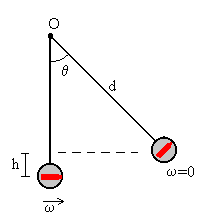
\includegraphics[width=0.7\textwidth]{balistico.png}
    \end{minipage}
  \item Propiedades elípticas: 
    \begin{enumerate}
      \item Verifique que el círculo, cuya expresión es $x^2 + y^2 = r^2$, pertenece a la familia de las elipses: 
        \[\left (\frac xa \right )^2  + \left ( \frac yb \right )^2 = 1, \]
        donde $a$ y $b$ son respectivamente el eje mayor y menor de la elipse.
      \item La excentricidad $\epsilon$ es una características de las cónicas y está dada por \[ \epsilon = \sqrt{1 - \frac{b^2}{a^2}} = \frac{\sqrt{a^2-b^2}}{a}.\] Utilizando las propiedades de la elipse, demuestre que la distancia $f$ entre el centro de la elipse y uno de los focos está dada por:
        \[f=a \, \epsilon = \sqrt{a^2 - b^2}\]
        Luego, muestre que la distancia mínima del foco a un punto de la órbita (llamada periápside) esta dada por $r_{pe} = (1-e) a$, mientras que la distancia máxima (apoápside) es $r_{ap}=(1+e) a$.
      \item Utilizando el {\emph{método del jardinero}}, construya una elipse que tenga $a=10$\,cm, y $b=5$\,cm.
    \end{enumerate}

\item Recordemos la primera ley de Kepler: 

``{\emph{Todos los planetas se desplazan alrededor del Sol describiendo órbitas
elípticas, estando el Sol situado en uno de sus focos}}'' 

Utilizando los valores del afelio, perihelio y excentricidad de Mercurio,
Venus, la Tierra, Urano y Plutón (utilizar la tabla de la guía 2), calcule para cada uno de ellos lo siguiente:

\begin{enumerate}
\item Los valores de $a$ y $b$ para cada una de las órbitas;
\item La distancia desde el ``{\emph{otro foco}}'' al Sol.
\end{enumerate}

\item Utilizando los períodos orbitales y las distancias al Sol para Venus, La Tierra, Marte, Júpiter, Saturno, Urano y Neptuno, verificaremos la tercera ley de Kepler,
  \[
    a^3 = k_{\mathrm{Sol}} T^2,
  \]
  donde $a$ es el eje mayor de la elipse (igual a la distancia media por las propiedades de las elipses), $T$ es el periodo del planeta, y $k$ es la constante de proporcionalidad y corresponde a, 
  \[
    k = \frac{G M_{\mathrm{Sol}}}{4 \pi^2}.
  \]

Para ello, grafique el cuadrado del período orbital, medido en días, como función del cubo de la distancia media al Sol, medida en millones de kilómetros.

La pendiente de la recta obtenida, $\Delta y / \Delta x$, no es otra que la constante de proporcionalidad $k_{\mathrm{Sol}}$. A partir de los resultados obtenidos, calcule el valor de $k$ en el sistema métrico internacional, y luego, utilizando este valor, calcule la masa del Sol. Compare el resultado obtenido con la masa tabulada del Sol, $M_\mathrm{Sol}=1.988\times10^{30}$\,kg.

\item Satélites
\begin{enumerate}
\item A partir de la expresión para la velocidad orbital de una órbita circular, 
  \[v_O = \frac{2 \pi r}{t},\]
usando la tercera ley de Kepler demuestre que para el caso circular la velocidad orbital vale: 
\[v_O = \sqrt{\frac{GM}{r}}. \]
dónde $G$ es la constante de gravitación universal, $M$ es la masa del cuerpo central, $r$ es el radio de la órbita y $T$ es el periodo orbital.
\item Calcule el radio $r$ para la órbita de un satélite geoestacionario ($T=24$\,horas).
\item Calcule la velocidad orbital de la estación espacial internacional, que se encuentra a una altura media de $330$\,km. Luego determine el tiempo requerido para completar una órbita.
\end{enumerate}

\item Un nuevo cometa de masa $m=10^{12}$\,kg fue descubierto en el sistema solar.
Luego de algunas mediciones, se supo que su órbita es elíptica y el perihelio
está situado a sólo $10^6$ km del Sol.

\begin{enumerate}
\item Calcule la distancia al Sol del afelio sabiendo que el período es de 10 años.
\item ¿Cuáles es el valor de la energía potencial en el perihelio y en el afelio?
\item Usando la segunda ley de Kepler, calcule la relación entre las energías
cinéticas en el afelio y en el perihelio (ayuda: suponga que las áreas barridas
son triangulares, $A=\frac{1}{2} b \times h$).
\end{enumerate}

\item Imagine que un planeta de masa $m=M_\mathrm{Tierra}$ orbita en torno a una estrella de
masa $M=6.5 \times 10^{30}$\,kg a una distancia media $r=4.5\times10^8$\,km. Usando
las leyes de Kepler, calcule el tiempo que requiere el planeta para completar
una órbita completa y su velocidad orbital media.

\item La órbita del planeta Mercurio es bastante alongada y posee una de las mayores
excentricidades del Sistema Solar, siendo sólo superada por Plutón. Las
distancias al Sol en su perihelio y afelio son:

Perihelio: $\overline{PE} = 45\,943\,700$\,km; Afelio $\overline{AF} =
69\,874\,671$\,km, respectivamente.
\begin{enumerate}
\item Calcule la excentricidad $\epsilon$ de la órbita y determine el valor de
los semiejes $a$ y $b$.
\item Se sabe que la cantidad de movimiento angular de Mercurio en su órbita es $L = 8.9585
\times 10^{38}$\,kg\,m$^2$\,s$^{-1}$. Calcule la velocidad del planeta en el
perihelio y en el afelio.
\item Usando la Tercera Ley de Kepler, determine el periodo $T$ del planeta.
\end{enumerate}
\end{enumerate}
\end{document}
%%%%
